\documentclass[12pt]{article}
\usepackage[lmargin=1in,rmargin=1in,tmargin=1in,bmargin=1in]{geometry}

\usepackage{aryaman}

\setcounter{tocdepth}{2}

\title{Linear Quotients of Connected Ideals of Graphs}
\author{Aryaman Maithani (Joint work with H. Ananthnarayan and Omkar Javadekar)}
\date{March 29, 2024}

\usepackage[
	hyperref = true,      	% Link to online documents
  	backend  = bibtex,      % Use bibtex instead of biber
  	sorting  = nyt,       	% Sorts by (name, year, title)
  	style  = alphabetic 	% Citations look like [Har77]
]{biblatex}
\addbibresource{talks.bib}

\begin{document}

\maketitle
% \tableofcontents

\section{Introduction}

Notes I made for my talk at the commutative algebra seminar at the University of Utah. I introduce the notions of linear resolutions and linear quotients, as well as some monomial ideals related to graphs. I mention our results of characterising when the connected ideals of trees have linear quotients, and giving a sufficient condition for general graphs. 

Throughout the article, $V$ will be a finite set, $G$ a finite simple graph with vertex set $V$, and $E$ its edge set. $K$ will denote a field.

We let $K[V] \vcentcolon= K[x_{v} : v \in V]$ be the polynomial ring over $K$ with variables indexed by elements of $V$. Given a subset $C \subset V$, we define the monomial
\begin{equation*} 
	x_{C} \vcentcolon= \prod_{c \in C} x_{c} \in K[V].
\end{equation*}

\section{Simplicial complexes, graphs, and Stanley-Reisner ideals}

Let $V$ be a finite set. A \deff{simplicial complex} $\Delta$ on $V$ is a collection of subsets of $V$ such that 
\begin{itemize}
	\item $G \in \Delta$ and $F \subset G$ implies $F \in \Delta$,
	\item $\{v\} \in \Delta$ for all $v \in V$.
\end{itemize}

The elements of $\Delta$ are called \deff{faces} and maximal faces (with respect to inclusion) are called \deff{facets}. Subsets of $V$ which are \emph{not} in $\Delta$ are called nonfaces (of $\Delta$).

\begin{ex}
	Our examples of interest will be simplicial complexes associated to (finite, simple) graphs. To begin with, let $G = (V, E)$ be a graph. Recall that a subset $C \subset V$ is said to be \deff{independent} is no two vertices in $C$ share an edge. Singletons are independent and being independence is closed under taking subsets, hence we get a simplicial complex:
	\begin{align*} 
		\Ind(G) \vcentcolon=&\ \{C \subset V : C \text{ is independent}\}.
	\end{align*}
	This is called the \deff{independence complex} of $G$.
\end{ex}

\begin{defn}
	 The \deff{Stanley-Reisner ideal (with respect to $K$)} of $\Delta$ is the ideal $I_{\Delta} \subset K[V]$ defined as
	\begin{align*} 
		I_{\Delta} \vcentcolon=&\, (x_{C} : C \text{ is a nonface}) \\
		=&\, (x_{C} : C \text{ is a minimal nonface}) \\
		=& \bigcap_{F \text{ a face}} (x_{v} : v \notin F) \\
		=& \bigcap_{F \text{ a facet}} (x_{v} : v \notin F) 
	\end{align*}
\end{defn}
The last equation is in fact a primary decomposition of $I_{\Delta}$.

\begin{ex} \label{ex:edge-ideal-and-dual}
	Turning back to our earlier example, we can examine what the Stanley-Reisner ideal of $\Ind(G)$ is. This is precisely what is known as the \deff{edge ideal} of the graph:
	\begin{align*} 
		I_{\Ind(G)} &= (x_{v} x_{w} : \{v, w\} \text{ is an edge}) \\
		&= (x_{e} : e \in E) =\vcentcolon I(G).
	\end{align*}
	This comes down to the observation that a minimal nonface of $\Ind(G)$ is precisely an edge.

	There is also the notion of a dual of a simplicial complex (equivalently, dual of a squarefree monomial ideal). For edge ideals, it takes the form
	\begin{equation*} 
		I(G)^{\vee} = I_{\Ind(G)^{\vee}} = \bigcap_{\{v, w\} \in E} (x_{v}, x_{w}).
	\end{equation*}
	The double-dual gives back the same object.
\end{ex}

\section{Linear resolutions and linear quotients}

Let $I$ be a homogeneous ideal generated by elements of degree $d$. Let $(\mathbb{F}_{\bullet}, \partial_{\bullet})$ be the minimal graded free resolution of $I$ (as a module). We say that $I$ has \deff{linear resolution} if any of the following equivalent conditions hold:
\begin{enumerate}[label=(\alph*)]
	\item The entries of $\partial_{i}$ for $i \ge 1$ are linear (or zero).
	\item The height of the Betti table of $I$ is $d$. 
	\item $\reg(I) = d$.
\end{enumerate}

\begin{ex}
	Consider the graph $G$ drawn as
	\begin{tikzpicture}
	\Vertex[style={minimum size=0.2cm,draw=black,fill=white,text=black,shape=circle},LabelOut=false,L=\hbox{$a$},x=0.5cm,y=1.0cm]{v0}
	\Vertex[style={minimum size=0.2cm,draw=black,fill=white,text=black,shape=circle},LabelOut=false,L=\hbox{$b$},x=0.0cm,y=0.0cm]{v1}
	\Vertex[style={minimum size=0.2cm,draw=black,fill=white,text=black,shape=circle},LabelOut=false,L=\hbox{$c$},x=1.0cm,y=0.0cm]{v2}
	%
	\Edge[lw=0.02cm,style={color=black,},](v0)(v1)
	\Edge[lw=0.02cm,style={color=black,},](v0)(v2)
	\Edge[lw=0.02cm,style={color=black,},](v1)(v2)
	%
	\end{tikzpicture}. We have $I(G) = (ab, bc, ca)$.

	Running this example on Macaulay2 gives the Betti table (over $K = \mathbb{F}_{7}$) of $I(G)$ as
	\begin{equation*} 
		\begin{matrix}
        & 0 & 1\\
	     \text{total:}
	        & 3 & 2\\
	     2: & 3 & 2
	     \end{matrix}
	\end{equation*}	

	Note that the resolution of a monomial ideal may depend on the characteristic\footnotemark.
\end{ex}
\footnotetext{as well as the version of Macaulay2 that you are using}

\begin{rem}
	The Stanley-Reisner ideal of the triangulation of $\mathbb{R}\mathbb{P}^{2}$ has the property of having linear resolutions precisely if the characteristic is two.
\end{rem}

\begin{thm}[{\cite[Theorem 3]{EagonReiner}}] \label{thm:eagon-reiner}
	$I_{\Delta}$ has linear resolution if and only if $K[V]/I_{\Delta^{\vee}}$ is Cohen-Macaulay.
\end{thm}

A running theme of questions is whether one can characterise ideals (among certain classes) that have linear resolution. After introducing some more terminology, we shall state a celebrated theorem of Fr\"{o}berg's that characterises squarefree quadratic monomials. 

We now introduce a stronger property for a monomial ideal to have: that of \emph{linear quotients}.

\begin{defn} \label{defn:linear-quotients}
	Let $I$ be a monomial ideal. We denote by $G(I)$ the unique minimal monomial system of generators of $I$. We say that $I$ has \deff{linear quotients}, if there exists an order $\sigma = u_{1}, \ldots, u_{m}$ on $G(I)$ such that the colon ideal $\langle u_{1}, \ldots, u_{i - 1} \rangle : \langle u_{i} \rangle$ is generated by a subset of the variables, for $i = 2, \ldots, m$. Any such order is said to be an \deff{admissible order}.
\end{defn}

\begin{rem}
	We immediately note that colons of monomial ideals and monomials are straightforward to compute. Indeed, the colon is generated by the ``pairwise colons'' which are again monomials.

	This also shows that the property of having linear quotients is characteristic-independent.
\end{rem}

\begin{thm}[\cite{JahanZheng}]
	Let $I$ be a monomial equigenerated in degree $d$. 
	\begin{equation*} 
		I \text{ has linear quotients} \Rightarrow I \text{ has linear resolution}.
	\end{equation*}
\end{thm}

\section{Some terminology about graphs}

Recall that a subgraph of a graph is a subcollection of vertices and a subcollection of edges between those vertices. A subgraph is said to be \deff{induced} if we pick all the edges between those vertices. 

\begin{ex} \label{ex:house-graph}
	Consider the \emph{house graph} $G$

	\begin{tikzpicture}
	\definecolor{cv0}{rgb}{0.0,0.0,0.0}
	\definecolor{cfv0}{rgb}{1.0,1.0,1.0}
	\definecolor{clv0}{rgb}{0.0,0.0,0.0}
	\definecolor{cv1}{rgb}{0.0,0.0,0.0}
	\definecolor{cfv1}{rgb}{1.0,1.0,1.0}
	\definecolor{clv1}{rgb}{0.0,0.0,0.0}
	\definecolor{cv2}{rgb}{0.0,0.0,0.0}
	\definecolor{cfv2}{rgb}{1.0,1.0,1.0}
	\definecolor{clv2}{rgb}{0.0,0.0,0.0}
	\definecolor{cv3}{rgb}{0.0,0.0,0.0}
	\definecolor{cfv3}{rgb}{1.0,1.0,1.0}
	\definecolor{clv3}{rgb}{0.0,0.0,0.0}
	\definecolor{cv4}{rgb}{0.0,0.0,0.0}
	\definecolor{cfv4}{rgb}{1.0,1.0,1.0}
	\definecolor{clv4}{rgb}{0.0,0.0,0.0}
	\definecolor{cv1v2}{rgb}{0.0,0.0,0.0}
	\definecolor{cv1v4}{rgb}{0.0,0.0,0.0}
	\definecolor{cv0v1}{rgb}{0.0,0.0,0.0}
	\definecolor{cv2v3}{rgb}{0.0,0.0,0.0}
	\definecolor{cv0v2}{rgb}{0.0,0.0,0.0}
	\definecolor{cv3v4}{rgb}{0.0,0.0,0.0}
	%
	\Vertex[style={minimum size=0.6cm,draw=cv0,fill=cfv0,text=clv0,shape=circle},LabelOut=false,L=\hbox{$a$},x=2.6671cm,y=3.0cm]{v0}
	\Vertex[style={minimum size=0.6cm,draw=cv1,fill=cfv1,text=clv1,shape=circle},LabelOut=false,L=\hbox{$b$},x=1.0473cm,y=1.9693cm]{v1}
	\Vertex[style={minimum size=0.6cm,draw=cv2,fill=cfv2,text=clv2,shape=circle},LabelOut=false,L=\hbox{$c$},x=3.0cm,y=1.5285cm]{v2}
	\Vertex[style={minimum size=0.6cm,draw=cv3,fill=cfv3,text=clv3,shape=circle},LabelOut=false,L=\hbox{$d$},x=2.1847cm,y=0.0cm]{v3}
	\Vertex[style={minimum size=0.6cm,draw=cv4,fill=cfv4,text=clv4,shape=circle},LabelOut=false,L=\hbox{$e$},x=0.0cm,y=0.4757cm]{v4}
	%
	\Edge[lw=0.06cm,style={color=cv1v2,},](v1)(v2)
	\Edge[lw=0.06cm,style={color=cv1v4,},](v1)(v4)
	\Edge[lw=0.06cm,style={color=cv0v1,},](v0)(v1)
	\Edge[lw=0.06cm,style={color=cv2v3,},](v2)(v3)
	\Edge[lw=0.06cm,style={color=cv0v2,},](v0)(v2)
	\Edge[lw=0.06cm,style={color=cv3v4,},](v3)(v4)
	%
	\end{tikzpicture}.

	$G$ contains the $4$-cycle as an induced subgraph. $G$ also contains the $5$-cycle as a subgraph, but not as an induced subgraph.
\end{ex}

A running theme is to restrict one's attention to graphs that don't contain a forbidden (family of) graph(s) as an induced subgraph and prove results about those. The celebrated result of Fr\"{o}berg is one example of this.

\begin{thm}[\cite{Froberg}]
	Let $G$ be a graph. The following are equivalent: 
	\begin{itemize}
		\item $I(G)$ has linear resolution.
		\item $G^{c}$ is chordal, i.e., contains no induced $n$-cycle for $n \ge 4$.
	\end{itemize}
\end{thm}
Note that since every squarefree monomial ideal is of the form $I(G)$, the above completely characterises linear resolution for such ideals. Combined with the following result, we also have the complete characterisation of such ideals with linear quotients.

\begin{thm}[{\cite[Theorem 3.2]{HerzogHibiZheng}}]
	Let $I$ be a monomial ideal equigenerated in degree $2$. The following are equivalent:
	\begin{enumerate}[label=(\alph*)]
		\item $I$ has a linear resolution.
		\item $I$ has linear quotients.
		\item Each power of $I$ has a linear resolution.
	\end{enumerate}
\end{thm}

On the other hand, combining this with \Cref{thm:eagon-reiner} gives us a way of telling when certain ideals define Cohen-Macaulay rings, perhaps best depicted with an example.

\begin{ex}
	Consider $I = (a, b) \cap (c, d)$. As noted in \Cref{ex:edge-ideal-and-dual}, $I^{\vee}$ is the edge ideal of \begin{tikzpicture}
	\definecolor{cv0}{rgb}{0.0,0.0,0.0}
	\definecolor{cfv0}{rgb}{1.0,1.0,1.0}
	\definecolor{clv0}{rgb}{0.0,0.0,0.0}
	\definecolor{cv1}{rgb}{0.0,0.0,0.0}
	\definecolor{cfv1}{rgb}{1.0,1.0,1.0}
	\definecolor{clv1}{rgb}{0.0,0.0,0.0}
	\definecolor{cv2}{rgb}{0.0,0.0,0.0}
	\definecolor{cfv2}{rgb}{1.0,1.0,1.0}
	\definecolor{clv2}{rgb}{0.0,0.0,0.0}
	\definecolor{cv3}{rgb}{0.0,0.0,0.0}
	\definecolor{cfv3}{rgb}{1.0,1.0,1.0}
	\definecolor{clv3}{rgb}{0.0,0.0,0.0}
	\definecolor{cv0v1}{rgb}{0.0,0.0,0.0}
	\definecolor{cv2v3}{rgb}{0.0,0.0,0.0}
	%
	\Vertex[style={minimum size=0.4cm,draw=cv0,fill=cfv0,text=clv0,shape=circle},LabelOut=false,L=\hbox{$a$},x=0.0cm,y=2.9837cm]{v0}
	\Vertex[style={minimum size=0.4cm,draw=cv1,fill=cfv1,text=clv1,shape=circle},LabelOut=false,L=\hbox{$b$},x=0.8175cm,y=0.0163cm]{v1}
	\Vertex[style={minimum size=0.4cm,draw=cv2,fill=cfv2,text=clv2,shape=circle},LabelOut=false,L=\hbox{$c$},x=2.3013cm,y=3.0cm]{v2}
	\Vertex[style={minimum size=0.4cm,draw=cv3,fill=cfv3,text=clv3,shape=circle},LabelOut=false,L=\hbox{$d$},x=3.0cm,y=0.0cm]{v3}
	%
	\Edge[lw=0.04cm,style={color=cv0v1,},](v0)(v1)
	\Edge[lw=0.04cm,style={color=cv2v3,},](v2)(v3)
	%
	\end{tikzpicture}.

	But the complement of the above graph is the $4$-cycle, which is not chordal. Thus, $I^{\vee}$ does not have a linear resolution and hence $K[V]/I$ is not Cohen-Macaulay. This can extended to any ideal $I$ which is given by intersection of ideals generated by two variables.
\end{ex}

\section{Higher analogues of the edge ideal}

We now look at some generalisations of the edge ideal. Let $G$ be a graph. For $t \ge 2$, define the two classes of ideals:
\begin{itemize}
	\item the \deff{$t$-path ideal} $I_{t}(G)$ is generated by the paths of $G$ of length $t$;
	\item the \deff{$t$-connected ideal} $J_{t}(G)$ is generated by the connected subsets of $G$ of size $t$.
\end{itemize}
(Recall that we can identify a subset $C \subset V(G)$ with the monomial $x_{C} \in K[V]$. That is what we mean by generated above.)

$J_{t}(G)$ seems to be a somewhat more natural analogue. For one, it is the Stanley-Reisner ideal of the simplicial complex $\Ind_{t - 1}(G)$, where
\begin{equation*} 
	\Ind_{r}(G) = \{C \subset V : \text{every connected component of $G[C]$ has size $\le r$}\}.
\end{equation*}
Note that $\Ind_{1}(G) = \Ind(G)$ and $I_{2}(G) = J_{2}(G) = I(G)$.

\begin{defn}
	We say that a graph $(V, E)$ is \deff{$t$-gap-free} if whenever $C$ and $C'$ are two disjoint connected subsets of $V$ of size $t$, then there is an edge joining a vertex of $C$ to a vertex of $C'$.
\end{defn}

\begin{rem}
	$J_{t}(G)$ can be viewed as an edge ideal of an associated \emph{hypergraph}. Using \cite[Theorem 1.4]{HaWoodroofe}, it is relatively straightforward to show that
	\begin{equation*} 
		J_{t}(G) \text{ has a linear resolution} \Rightarrow \text{$G$ is $t$-gap-free}.
	\end{equation*}
	(See \cite[Corollary 4.3]{AnanthnarayanJavadekarMaithani}.)

	This project began as an attempt to prove the converse.
\end{rem}

\begin{thm}[\cite{AnanthnarayanJavadekarMaithani}] \label{thm:theorem-for-trees}
	Let $T$ be a tree, i.e., a connected graph with no cycles. For each $t \ge 2$, the following are equivalent.
	\begin{enumerate}[label=(\alph*)]
		\item $J_{t}(T)$ has linear quotients.
        \item $J_{t}(T)$ has a linear resolution.
        \item $T$ is $t$-gap-free
	\end{enumerate}
\end{thm}
Note that for $t = 2$, we recover Fr\"{o}berg's result for trees.

The above does not hold in general. Indeed, $C_{5}$ is ($2$-)gap-free but $J_{2}(C_{5})$ does not have linear resolution, for it is not co-chordal. In fact, we showed that every ($\ge 5$)-cycle is a counterexample to the above for a suitable $t$ (\cite[Theorem 5.2]{AnanthnarayanJavadekarMaithani}).

\begin{proof}[Sketch for \Cref{thm:theorem-for-trees}]
	We prove this by induction on $\md{V(T)}$. If $\md{V(T)} = t$, this is clear. Assume $\md{V(T)} > t$. \newline
	Let $\ell$ be a leaf of $T$. Then, $T \setminus \{\ell\}$ is an induced subgraph and hence, $t$-gap-free. By hypothesis, there is an admissible order on $G(J_{t}(T \setminus \{\ell\}))$ (recall \Cref{defn:linear-quotients}). Furthermore,
	\begin{equation*} 
		G(J_{t}(T)) = G(J_{t}(T \setminus \{\ell\})) \sqcup \{\text{connected subsets of size $t$ containing $\ell$}\}.
	\end{equation*}
	We showed in the paper that appending the extra generators in any order gives an admissible order.
\end{proof}

Continuing the theme of prohibiting certain subgraphs, we introduce some more terminology: Recall that $K_{1, t}$ is the graph with $V = \{0, \ldots, t\}$ and $E = \{(0, i) : 1 \le i \le t\}$.
\begin{defn}
	A graph is called \deff{$t$-claw-free} if it contains no induced subgraph isomorphic to $K_{1, t}$.
\end{defn}

For path ideals, Banerjee showed the following.
\begin{thm}[\cite{Banerjee}]
	If $G$ is a (2-)gap-free and (3-)claw-free graph, then $I_{t}(G)$ has linear resolution for all $t \ge 3$.
\end{thm}

\begin{thm}[\cite{AnanthnarayanJavadekarMaithani}]
	Let $t \ge 3$ be an integer. Suppose $G$ is a gap-free and $t$-claw-free graph. Then, $J_{t}(G)$ has linear quotients. In particular, $J_{t}(G)$ has a linear resolution.
\end{thm}

\printbibliography
\end{document}